\documentclass[12pt]{article}

\usepackage{amsfonts, amsmath, amssymb, amsthm, dsfont, enumitem, fancyhdr, graphicx, mathtools, tikz-cd}
\usepackage[margin=0.85in, includehead, includefoot, heightrounded]{geometry}
\allowdisplaybreaks
\pagestyle{fancy}
\rhead{Erick Lin}

\newcommand{\norm}[1]{\left\lVert#1\right\rVert}
\newcommand*\dist{\mathop{\!\mathrm{d}}}
\DeclareMathOperator{\im}{Im}
%\let\ker\relax %RedeclareMathOperator
%\DeclareMathOperator{\ker}{Ker}
\DeclareMathOperator{\Hom}{Hom}
\DeclareMathOperator{\Ext}{Ext}
\renewcommand{\thesubsection}{\arabic{subsection}}
\newcommand*\sq{\mathbin{\vcenter{\hbox{\rule{.4ex}{.4ex}}}}}
\newcommand{\iso}{\approx}
\newcommand{\RP}{\mathbb{R}\mathrm{P}}
\newtheorem{theorem}{Theorem}
\newtheorem{lemma}[theorem]{Lemma}

\begin{document}

\section*{MATH 6441 -- HW8 Solutions}
\subsection*{Section 3.1}
\begin{enumerate}
    \item[5.]
        \boldmath\textbf{Regarding a cochain $\varphi \in C^1(X; G)$ as a function from paths in $X$ to $G$, show that if $\varphi$ is a cocycle, then
        }\unboldmath \par
        \begin{enumerate}
            \item
                \boldmath\textbf{$\varphi(f \sq g) = \varphi(f) + \varphi(g)$,
                }\unboldmath \par
                Define $\sigma : \Delta^2 \to X$ as the function composition of projecting $\Delta^2 = [v_0, v_1, v_2]$ onto the edge $[v_0, v_2]$ (so that $v_1$ maps to the midpoint of $[v_0, v_1]$) and then mapping via $f \sq g : [v_0, v_2] \to X$; we can see that $\sigma|_{[v_0, v_1]} = f$, $\sigma|_{[v_1, v_2]} = g$, and $\sigma|_{[v_0, v_2]} = f \sq g$. Thus,
                \begin{align*}
                    \partial\sigma = \sigma|_{[v_0, v_1]} - \sigma|_{[v_0, v_2]} + \sigma|_{[v_1, v_2]} = f - f \sq g + g
                \end{align*}
                and because $\varphi$ being a cocycle implies $\delta\varphi = \varphi\partial = 0$,
                \begin{align*}
                    \varphi(f \sq g) = \varphi(f + g - \partial\sigma) = \varphi(f) + \varphi(g).
                \end{align*}

            \item
                \boldmath\textbf{$\varphi$ takes the value 0 on constant paths,
                }\unboldmath \par
                \iffalse
                    Define $\sigma : \Delta^2 \to X$ as the composition of projecting $[v_0, v_1, v_2]$ onto the edge $[v_0, v_2]$ and then mapping via $[v_0, v_2] \to \{c\}$ where $c$ is a constant, so that
                    \begin{align*}
                        \partial\sigma = \sigma|_{[v_0, v_1]} - \sigma|_{[v_0, v_2]} + \sigma|_{[v_1, v_2]} = c - c + c = c.
                    \end{align*}
                    Therefore,
                    \begin{align*}
                        0 = \varphi(\partial\sigma) = \varphi(c).
                    \end{align*}
                \fi
                If $c$ is a constant path on $X$, then from (a) we have $\varphi(c \sq c) = \varphi(c) + \varphi(c)$. But $c \sq c = c$, giving $\varphi(c) = 0$.

            \item
                \boldmath\textbf{$\varphi(f) = \varphi(g)$ if $f \simeq g$,
                }\unboldmath \par
                \iffalse
                    Define $\sigma : \Delta^2 \to X$ as the composition of projecting $[v_0, v_1, v_2]$ onto the edge $[v_0, v_2]$ and then mapping via (assuming the homotopy fixes the endpoints) $f \sq \overline{g} : [v_0, v_2] \to X$, so that
                    \begin{align*}
                        \partial\sigma = \sigma|_{[v_0, v_1]} - \sigma|_{[v_0, v_2]} + \sigma|_{[v_1, v_2]} = f - f \sq \overline{g} + \overline{g}
                    \end{align*}
                \fi
                Assuming the homotopy $H : I \times I \to X$ fixes the endpoints, we have that $f(0) = H(0, t) = g(0)$ and $f(1) = H(1, t) = g(1)$ for all $t \in [0, 1]$. \\
                \vspace{2.5cm} \\
                From the diagram,
                \begin{align*}
                    \partial[g(0), g(1), f(1)] &= [g(0), g(1)] - [g(0), f(1)] + [g(1), f(1)] = g - h - H(1, t) \\
                    \partial[f(0), f(1), g(0)] &= [f(0), f(1)] - [f(0), g(0)] + [f(1), g(0)] = f + H(0, t) - h.
                \end{align*}
                $\delta\varphi = \varphi\partial = 0$, and $\varphi(H(0, t)) = \varphi(H(1, t)) = 0$ by (b), so we have
                \begin{align*}
                    0 = \varphi\partial[g(0), g(1), f(1)] = \varphi(g - h - H(1, t)) = \varphi(g) - \varphi(h) \\
                    0 = \varphi\partial[f(0), f(1), g(0)] = \varphi(f + H(0, t) - h) = \varphi(f) - \varphi(h),
                \end{align*}
                and thus $\varphi(f) = \varphi(g)$.

            \item
                \boldmath\textbf{$\varphi$ is a coboundary iff $\varphi(f)$ depends only on the endpoints of $f$, for all $f$.
                }\unboldmath \par
                ($\Rightarrow$) We have that $\varphi = \delta\psi$ for some cochain $\psi \in C^0(X; G)$, and thus the quantity
                \begin{align*}
                    \varphi(f) = \delta\psi(f) = \psi(\partial f) = \psi(f(1)) - \psi(f(0))
                \end{align*}
                depends only on $f(0)$ and $f(1)$. \par
                ($\Leftarrow$) Any $\psi \in C^0(X, G)$ is a function from points in $X$ to $G$, so if we define $\psi$ such that $\psi(f(0))$ is an arbitrary value and $\psi(f(1)) = \varphi(f) + \psi(f(0))$, then
                \begin{align} \label{eq:f}
                    \varphi(f) = \psi(f(1)) - \psi(f(0)).
                \end{align}
                $f$ is well-defined because we are given that $\varphi(f)$ depends only on the endpoints of $f$. (\ref{eq:f}) then becomes
                \begin{align*}
                    \psi(f(1) - f(0)) = \psi(\partial f) = \delta\psi(f),
                \end{align*}
                and since $f$ was arbitrary, we have that $\varphi = \delta\psi$, so $\varphi$ is a coboundary.
        \end{enumerate}
        \boldmath\textbf{[In particular, (a) and (c) give a map $H^1(X; G) \to \Hom(\pi_1(X), G)$, which the universal coefficient theorem says is an isomorphism if $X$ is path-connected.]
        }\unboldmath \par

    \item[6.]
        \begin{enumerate}
            \item
                \boldmath\textbf{Directly from the definitions, compute the simplicial cohomology groups of $S^1 \times S^1$ with $\mathbb{Z}$ and $\mathbb{Z}_2$ coefficients, using the $\Delta$-complex structure.
                }\unboldmath \par
                {\centering
                    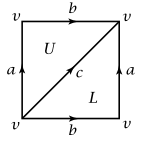
\includegraphics[scale=1]{torus_delta}
                \\}
                The $\Delta$-complex structure has one vertex $v$, three edges $a, b$, and $c$, and two $2$-simplices $U$ and $L$.
                \iffalse
                    Before computing the simplicial cochain groups for each coefficient, we state the following lemma:
                    \begin{lemma}
                        $\Hom(\mathbb{Z}, A) \iso A$ for any abelian group $A$.
                    \end{lemma}
                    \begin{proof}
                        $\mathbb{Z}$ is the free abelian group generated by the element $1$. Since homomorphisms are specified by where they send generators, each homomorphism can be identified to the element of $A$ to which $1$ is sent.
                    \end{proof}
                    By the lemma, we have that
                    \begin{gather*}
                        \Delta^0(K; \mathbb{Z}) = \Hom(\Delta_0(K), \mathbb{Z}) \iso \Hom(\mathbb{Z}, \mathbb{Z}) \iso \mathbb{Z} \\
                        \Delta^0(K; \mathbb{Z}^2) = \Hom(\Delta_0(K), \mathbb{Z}^2) \iso \Hom(\mathbb{Z}, \mathbb{Z}^2) \iso \mathbb{Z}^2 \\
                        \Delta^1(K; \mathbb{Z}) = \Hom(\Delta_1(K), \mathbb{Z}) \iso \Hom(\mathbb{Z}^3, \mathbb{Z}) \iso \mathbb{Z} \\
                        \Delta^1(K; \mathbb{Z}^2) = \Hom(\Delta_1(K), \mathbb{Z}^2) \iso \Hom(\mathbb{Z}^3, \mathbb{Z}^2) \iso \mathbb{Z}^2 \\
                        \Delta^2(K; \mathbb{Z}) = \Hom(\Delta_2(K), \mathbb{Z}) \iso \Hom(\mathbb{Z}^2, \mathbb{Z}) \iso \mathbb{Z} \\
                        \Delta^2(K; \mathbb{Z}^2) = \Hom(\Delta_2(K), \mathbb{Z}^2) \iso \Hom(\mathbb{Z}^2, \mathbb{Z}^2) \iso \mathbb{Z}^2.
                    \end{gather*}
                \fi
                For general $G$ coefficients, the simplicial cochain groups are given by $\Delta^n(S^1 \times S^1; G) = \Hom(\Delta_n(S^1 \times S^1), G)$, which are more specifically
                \begin{align*}
                    \Delta^0(S^1 \times S^1; G) &= \langle v^* : v \mapsto 1 \rangle \\
                    \Delta^1(S^1 \times S^1; G) &= \langle a^* : a \mapsto 1, b^* : b \mapsto 1, c^* : c \mapsto 1 \rangle \\
                    \Delta^2(S^1 \times S^1; G) &= \langle U^* : U \mapsto 1, L^* : L \mapsto 1 \rangle
                \end{align*}
                (where $x^* : x \mapsto 1$, or simply $x^*$, is the homomorphism that sends $x$ to $1$ and all other elements to $0$). \par
                %$\partial_1 = 0$ since $\partial a = \partial b = \partial c = v - v = 0$, so for all $f \in \Delta^0(S^1 \times S^1, \mathbb{Z})$, $\delta_0 f = f \partial_1 = 0$ and so $\delta_0 = 0$.
                %We know from the cochain complex that $\delta_0 = 0$.
                We now compute the coboundaries. First, $\delta_0 v^*(a) = v^* \partial_1(a) = v^*(v - v) = 0$, and likewise $\delta_0 v^*(b) = \delta_0 v^*(c) = 0$. Since we know that
                \begin{align*}
                    \delta_0 v^* = n_1 a^* + n_2 b^* + n_3 c^* \text{ where $n_i \in G$},
                \end{align*}
                we also have that $\delta_0 v^*(a) = n_1 a^*(a) + n_2 b^*(a) + n_3 b^*(a) = n_1 + 0 + 0 = n_1$, so substitution gives $n_1 = 0$. Similarly, $n_2 = n_3 = 0$, and so $\delta_0 v^* = 0$. \par
                Next, since $\partial_2 U = \partial_2 L = a + b - c$, $\delta_1 a^*(U) = a^* \partial_2(U) = a^*(a + b - c) = 1 + 0 - 0 = 1 = \delta_1 a^*(L)$ and similarly, $\delta_1 b^*(U) = b^*(a + b - c) = 1 = \delta_1 b^*(L)$ and $\delta_1 c^*(U) = c^*(a + b - c) = -1 = \delta_1 c^*(L)$. Since $\delta_1 a^*$, $\delta_1 b^*$, and $\delta_1 c^*$ are linear combinations of $U^*$ and $L^*$ with coefficients in $G$, following the same procedure as above gives $\delta_1 a^* = U^* + L^*$, $\delta_1 b^* = U^* + L^*$, and $\delta_1 c^* = -U^* - L^*$. The procedure in general gives us the following lemma:
                \begin{lemma} \label{lem:duality}
                    \sloppy
                    Given a topological space $X$ with $\Delta_n(X) = \langle x_1, \cdots, x_k \rangle$, $\Delta_{n + 1}(X) = \langle y_1, \cdots, y_m \rangle$, and
                    \begin{align*}
                        \partial_{n + 1} y_i = n_{i, 1} x_1 + n_{i, 2} x_2 + \cdots + n_{i, k} x_k, \quad 1 \leq i \leq m
                    \end{align*}
                    where $n_{i, j} \in \mathbb{Z}$, we have that
                    \begin{align*}
                        \delta_n x_j^* = n_{1, j}^* y_1^* + n_{2, j}^* y_2^* + \cdots + n_{m, j}^* y_m^*, \quad 1 \leq j \leq k
                    \end{align*}
                    where $n_{i, j}^*$ is the image of $n_{i, j}$ under the homomorphism $\mathbb{Z} \to G$ that sends the generator $1$ of $\mathbb{Z}$ to a generator of $G$.
                \end{lemma}
                Since there are no 3-simplices, $\delta_2 U^* = \delta_2 L^* = 0$. \par
                We can now see that for both $G = \mathbb{Z}$ and $G = \mathbb{Z}_2$, $H_\Delta^0(S^1 \times S^1; G) \iso \ker\delta_0 \iso \Delta^0(S^1 \times S^1; G) \iso G$, $H_\Delta^1(S^1 \times S^1; G) = \ker\delta_1 / \im\delta_0 \iso \ker\delta_1 \iso \langle a^* - b^*, a^* + c^* \rangle \iso G \oplus G$, and $H_\Delta^2(S^1 \times S^1; G) = \ker\delta_2 / \im\delta_1 \iso \Delta^2(S^1 \times S^1; G) / \langle U^* + L^* \rangle \iso \langle U^*, U^* + L^* \rangle / \langle U^* + L^* \rangle \iso \langle U^* \rangle \iso G$.
                In conclusion, the simplicial cohomology groups are given by
                \begin{align*}
                    H_\Delta^n(S^1 \times S^1; \mathbb{Z}) \iso \begin{cases}
                        \mathbb{Z} &\text{for } n = 0, 2 \\
                        \mathbb{Z} \oplus \mathbb{Z} &\text{for } n = 1 \\
                        0 &\text{for } n \geq 3
                    \end{cases}
                \end{align*}
                and
                \begin{align*}
                    H_\Delta^n(S^1 \times S^1; \mathbb{Z}_2) \iso \begin{cases}
                        \mathbb{Z}_2 &\text{for } n = 0, 2 \\
                        \mathbb{Z}_2 \oplus \mathbb{Z}_2 &\text{for } n = 1 \\
                        0 &\text{for } n \geq 3
                    \end{cases}.
                \end{align*}

            \item
                \boldmath\textbf{Do the same for $\RP^2$ and the Klein bottle.
                }\unboldmath \par
                {\centering
                    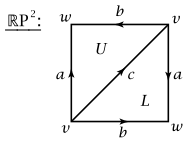
\includegraphics[scale=1]{rp2_delta}
                    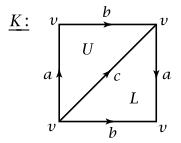
\includegraphics[scale=1]{klein_delta}
                \\}
                For $\RP^2$, the $\Delta$-complex structure has two vertices $v$ and $w$, three edges $a$, $b$, and $c$, and two $2$-simplices $U$ and $L$. For general $G$ coefficients, the simplicial cochain groups are given by $\Delta^n(\RP^2; G) = \Hom(\Delta_n(\RP^2), G)$, or more specifically $\Delta^0(\RP^2; G) = \langle v^*, w^* \rangle$, $\Delta^1(\RP^2; G) = \langle a^*, b^*, c^* \rangle$, and $\Delta^2(\RP^2; G) = \langle U^*, L^* \rangle$. \par
                We have that $\partial_1 a = w - v$, $\partial_1 b = w - v$, $\partial_1 c = v - v = 0$, $\partial_2 U = a - b - c$, and $\partial_2 L = a - b + c$, which by Lemma \ref{lem:duality} implies that $\delta_0 v^* = -a^* - b^*$, $\delta_0 w^* = a^* + b^*$, $\delta_1 a^* = U^* + L^*$, $\delta_1 b^* = -U^* - L^*$, $\delta_1 c^* = -U^* + L^*$, and $\delta_2 U^* = \delta_2 L^* = 0$. \par
                For both $G = \mathbb{Z}$ and $G = \mathbb{Z}_2$, $H_\Delta^0(\RP^2; G) \iso \ker\delta_0 = \langle v^* + w^* \rangle \iso G$. On the other hand,
                \begin{align*}
                    H_\Delta^1(\RP^2; G) &\iso \ker\delta_1 / \im\delta_0 \\
                    &\iso \begin{cases}
                        \langle a^* + b^* \rangle / \langle a^* + b^* \rangle \iso 0, &G = \mathbb{Z} \\
                        \langle a^* + b^*, a^* + c^* \rangle / \langle a^* + b^* \rangle \iso \langle a^* + c^* \rangle \iso G, &G = \mathbb{Z}_2
                    \end{cases}
                \end{align*}
                and
                \begin{align*}
                    H_\Delta^2(\RP^2; G) &= \ker\delta_2 / \im\delta_1 = \Delta^2(\RP^2; G) / \im\delta_1 \\
                    &\iso \begin{cases}
                        \langle L^*, U^* + L^* \rangle / \langle U^* + L^*, 2L^* \rangle \iso \langle L^* \rangle / \langle 2L^* \rangle \iso G/2G, &G = \mathbb{Z} \\
                        \langle L^*, U^* + L^* \rangle / \langle U^* + L^* \rangle \iso \langle L^* \rangle \iso G, &G = \mathbb{Z}_2
                    \end{cases}.
                \end{align*}
                In conclusion, the simplicial cohomology groups of $\RP^2$ are given by
                \begin{align*}
                    H_\Delta^n(\RP^2, \mathbb{Z}) \iso \begin{cases}
                        \mathbb{Z} &\text{for } n = 0 \\
                        \mathbb{Z}_2 &\text{for } n = 2 \\
                        0 &\text{otherwise}
                    \end{cases}
                \end{align*}
                and
                \begin{align*}
                    H_\Delta^n(\RP^2, \mathbb{Z}_2) \iso \begin{cases}
                        \mathbb{Z}_2 &\text{for } 0 \leq n \leq 2 \\
                        0 &\text{for } n \geq 3
                    \end{cases}.
                \end{align*}
                For $K$, the $\Delta$-complex structure has one vertex $v$, three edges $a$, $b$, and $c$, and two $2$-simplices $U$ and $L$. For general $G$ coefficients, the simplicial cochain groups are given by $\Delta^n(K; G) = \Hom(\Delta_n(K), G)$, or more specifically $\Delta^0(K; G) = \langle v^* \rangle$, $\Delta^1(K; G) = \langle a^*, b^*, c^* \rangle$, and $\Delta^2(K; G) = \langle U^*, L^* \rangle$. \par
                We have that $\partial_1 a = \partial b = \partial c = v - v = 0$, $\partial_2 U = a + b - c$, and $\partial_2 L = a - b + c$, which by Lemma \ref{lem:duality} implies that $\delta_0 v^* = 0$, $\delta_1 a^* = U^* + L^*$, $\delta_1 b^* = U^* - L^*$, $\delta_1 c^* = -U^* + L^*$, and $\delta_2 U^* = \delta_2 L^* = 0$. \par
                For both $G = \mathbb{Z}$ and $G = \mathbb{Z}_2$, $H_\Delta^0(K; G) \iso \ker\delta_0 = \langle v^* \rangle \iso G$. On the other hand,
                \begin{align*}
                    H_\Delta^1(K; G) &\iso \ker\delta_1 / \im\delta_0 \iso \ker\delta_1 \\
                    &\iso \begin{cases}
                        \langle b^* + c^* \rangle \iso G, &G = \mathbb{Z} \\
                        \langle a^* + b^*, b^* + c^* \rangle \iso G \oplus G, &G = \mathbb{Z}_2
                    \end{cases}
                \end{align*}
                and
                \begin{align*}
                    H_\Delta^2(K; G) &= \ker\delta_2 / \im\delta_1 = \Delta^2(K; G) / \im\delta_1 \\
                    &\iso \begin{cases}
                        \langle U^*, U^* + L^* \rangle / \langle U^* + L^*, 2U^* \rangle \iso \langle U^* \rangle / \langle 2U^* \rangle \iso G/2G, &G = \mathbb{Z} \\
                        \langle U^*, U^* + L^* \rangle / \langle U^* + L^* \rangle \iso \langle U^* \rangle \iso G, &G = \mathbb{Z}_2
                    \end{cases}.
                \end{align*}
                In conclusion, the simplicial cohomology groups of $K$ are given by
                \begin{align*}
                    H_\Delta^n(K; \mathbb{Z}) \iso \begin{cases}
                        \mathbb{Z} &\text{for } n = 0, 1 \\
                        \mathbb{Z}_2 &\text{for } n = 2 \\
                        0 &\text{for } n \geq 3
                    \end{cases}
                \end{align*}
                and
                \begin{align*}
                    H_\Delta^n(K; \mathbb{Z}_2) \iso \begin{cases}
                        \mathbb{Z}_2 &\text{for } n = 0, 2 \\
                        \mathbb{Z}_2 \oplus \mathbb{Z}_2 &\text{for } n = 1 \\
                        0 &\text{for } n \geq 3
                    \end{cases}.
                \end{align*}
        \end{enumerate}

    %http://at.yorku.ca/cgi-bin/bbqa?forum=ask_an_algebraic_topologist&task=show_msg&msg=2130.0001
    %http://homepages.math.uic.edu/~bshipley/548.08.hw3.pdf
    \item[11.]
        \boldmath\textbf{Let $X$ be the Moore space $M(\mathbb{Z}_m, n)$ obtained from $S^n$ by attaching a cell $e^{n + 1}$ by a map of degree $m$.
        }\unboldmath
        \begin{enumerate}
            \item
                \boldmath\textbf{Show that the quotient map $X \to X/S^n = S^{n + 1}$ induces the trivial map on $\tilde{H}_i(-; \mathbb{Z})$ for all $i$, but not on $H^{n + 1}(-; \mathbb{Z})$. Deduce that the splitting in the universal coefficient theorem for cohomology cannot be natural.
                }\unboldmath \par
                The cellular chain complexes are given by
                \begin{center}
                    \begin{tikzcd}
                        \cdots\arrow{r} & 0\arrow{r}\arrow{d} & \mathbb{Z}\arrow{r}{m}\arrow{d} & \mathbb{Z}\arrow{r}\arrow{d} & 0\arrow{r} & \cdots \\
                        \cdots\arrow{r} & 0\arrow{r} & \mathbb{Z}\arrow{r} & 0\arrow{r} & 0\arrow{r} & \cdots
                    \end{tikzcd}
                \end{center}
                We know that $H_i(X) \iso \mathbb{Z}_m$ if $i = n$ and $\tilde{H}_i(X) = 0$ for $i \neq n$, and also that $H_i(S^{n + 1}) \iso \mathbb{Z}$ if $i = n + 1$ and $\tilde{H}_i(S^{n + 1}) = 0$ for $i \neq n + 1$. Since at least one of $\tilde{H}_i(X)$ or $\tilde{H}_i(S^{n + 1})$ is trivial for all $i \geq 0$, the induced map $f_*$ is trivial. \par
                On the other hand, the cellular cochain complex at the $(n + 1)$st level is given by
                \begin{center}
                    \begin{tikzcd}
                        0 & \arrow{l}\mathbb{Z} & \arrow{l}[swap]{m}\mathbb{Z} \\
                        0 & \arrow{l}\mathbb{Z}\arrow[u, "f^\sharp"] & \arrow{l}0
                    \end{tikzcd}
                \end{center}
                where the top row is the cochain for $X$ and the bottom is the cochain for $S^{n + 1}$. Since $f$ induces a homeomorphism from the $(n + 1)$st cell of $X$ onto the $(n + 1)$st cell of $S^{n + 1}$, $f^\sharp$ is the identity map in degree $n + 1$, which induces the surjective map $\mathbb{Z} \to \mathbb{Z}_m$ on $H^{n + 1}(-; \mathbb{Z})$. Here, the splitting is not natural. \par
                In general, the sequences generated by the universal coefficient theorem for cohomology are given by
                \begin{center}
                    \begin{tikzcd}
                        0\arrow{r} & \Ext(H_n(X), \mathbb{Z})\arrow{r} & H^{n + 1}(X; \mathbb{Z})\arrow{r} & \Hom(H_{n + 1}(X), \mathbb{Z})\arrow{r} & 0 \\
                        0\arrow{r} & \Ext(H_n(S^{n + 1}), \mathbb{Z})\arrow{r}\arrow{u} & H^{n + 1}(S^{n + 1}; \mathbb{Z})\arrow{r}\arrow{u} & \Hom(H_{n + 1}(S^{n + 1}), \mathbb{Z})\arrow{r}\arrow{u} & 0,
                    \end{tikzcd}
                \end{center}
                which is not natural because otherwise, there would exist a map from $\Hom(H_{n + 1}(-), \mathbb{Z}$ to $H^{n + 1}(-; \mathbb{Z})$ making the diagram commutative, but composition is trivial in one direction and nontrivial in the other.

            \item
                \boldmath\textbf{Show that the inclusion $S^n \xhookrightarrow{} X$ induces the trivial map on $\tilde{H}^i(-; \mathbb{Z})$ for all $i$, but not on $H_n(-; \mathbb{Z})$.
                }\unboldmath \par
                If $g$ is the inclusion map, then the commutative diagram obtained by the universal coefficient theorem is given by
                \begin{center}
                    \begin{tikzcd}
                        0\arrow{r} & \Ext(\tilde{H}_{j - 1}(X), \mathbb{Z})\arrow{r}\arrow[d, "g^\sharp"] & \tilde{H}^j(X; \mathbb{Z})\arrow{r}\arrow[d, "g^*"] & \Hom(\tilde{H}_j(X), \mathbb{Z})\arrow{r}\arrow{d} & 0 \\
                        0\arrow{r} & \Ext(\tilde{H}_{j - 1}(S^n), \mathbb{Z})\arrow{r} & \tilde{H}^j(S^n; \mathbb{Z})\arrow{r} & \Hom(\tilde{H}_j(S^n), \mathbb{Z})\arrow{r} & 0,
                    \end{tikzcd}
                \end{center}
                Because $\tilde{H}_j(X)$ is isomorphic to either $\mathbb{Z}_m$ or 0, $\Hom(\tilde{H}_j(X), \mathbb{Z}) = 0$, and because $\tilde{H}_{j - 1}(S^n)$ is isomorphic to either $\mathbb{Z}$ or 0, $\Ext(\tilde{H}_{j - 1}(S^n)) = 0$. Thus, from the diagram above, $\Ext(\tilde{H}_{j - 1}(X), \mathbb{Z}) \cong \tilde{H}^j(X; \mathbb{Z})$ and $\tilde{H}^j(S^n; \mathbb{Z}) \cong \Hom(\tilde{H}_j(S^n), \mathbb{Z})$, and by commutativity, the composition of the latter isomorphism with either $g^\sharp$ and $g^*$ is zero. Because of the former isomorphism, $g^*$ must be the trivial map. \par
                $g$ maps the $n$-cell of $S^n$ homeomorphically onto the $n$-cell of $X$, so the induced chain map $g_\sharp$ is the identity map in degree $n$, inducing the surjective map $\mathbb{Z} \to \mathbb{Z}_m$ when $H_n(-) = H_n(-, \mathbb{Z})$ is applied.
        \end{enumerate}
\end{enumerate}
\end{document}
